\subsubsection{My-vimar-integration}

\begin{center}
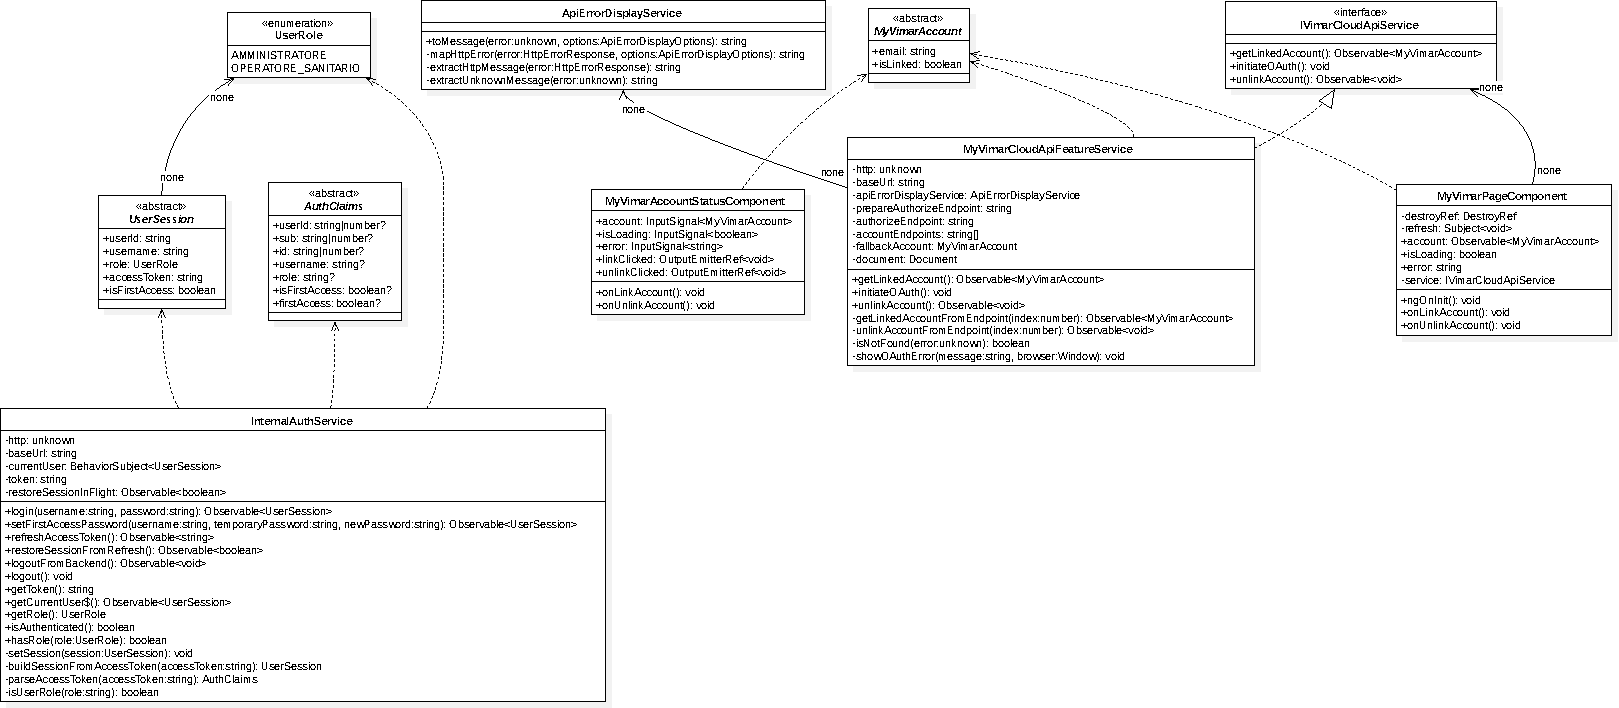
\includegraphics[width=\textwidth]{./frontend/my-vimar-integration/my-vimar-integration.pdf}
\captionof{figure}{Diagramma delle classi del modulo MyVimar integration}
\end{center}


\addAtr{+}{account: InputSignal$<$MyVimarAccount$>$}{Input obbligatorio che riceve i dati dell'account MyVimar.}
\addAtr{+}{isLoading: InputSignal$<$boolean$>$}{Input che indica se il caricamento dello stato è in corso.}
\addAtr{+}{error: InputSignal$<$string$>$}{Input che contiene il messaggio di errore relativo allo stato dell'account.}
\addAtr{+}{linkClicked: OutputEmitterRef$<$void$>$}{Output che emette un evento quando si clicca per collegare l'account.}
\addAtr{+}{unlinkClicked: OutputEmitterRef$<$void$>$}{Output che emette un evento quando si clicca per scollegare l'account.}
\addMet{+}{onLinkAccount() : void}{Emette l'evento linkClicked per avviare il collegamento dell'account MyVimar.}
\addMet{+}{onUnlinkAccount() : void}{Emette l'evento unlinkClicked per avviare lo scollegamento dell'account MyVimar.}
\makeCl{MyVimarAccountStatusComponent}{Il componente MyVimarAccountStatusComponent visualizza lo stato dell'account MyVimar, gestendo input per dati e stati di caricamento. Fornisce output per eventi di collegamento e scollegamento, facilitando l'interazione utente con l'integrazione MyVimar.}

\addAtr{-}{destroyRef: DestroyRef}{Riferimento per la gestione della distruzione del componente.}
\addAtr{-}{refresh\$: Subject$<$void$>$}{Subject per triggerare il refresh dello stato dell'account.}
\addAtr{+}{account\$: Observable$<$MyVimarAccount$>$}{Observable che emette lo stato corrente dell'account MyVimar.}
\addAtr{+}{isLoading: boolean}{Indica se un'operazione di caricamento è in corso.}
\addAtr{+}{error: string}{Messaggio di errore relativo alle operazioni MyVimar.}
\addAtr{-}{service: IVimarCloudApiService}{Servizio per l'interazione con l'API cloud di Vimar.}
\addMet{+}{ngOnInit() : void}{Inizializza l'observable per il recupero dello stato dell'account MyVimar con gestione errori.}
\addMet{+}{onLinkAccount() : void}{Avvia il processo di collegamento dell'account MyVimar tramite OAuth.}
\addMet{+}{onUnlinkAccount() : void}{Rimuove il collegamento dell'account MyVimar e aggiorna lo stato con gestione errori.}
\makeCl{MyVimarPageComponent}{Il componente MyVimarPageComponent gestisce la pagina di integrazione MyVimar, visualizzando lo stato dell'account e permettendo collegamento e scollegamento. Utilizza observable per gestire aggiornamenti reattivi e gestisce errori di comunicazione con l'API.}

\addAtr{+}{email: string}{}
\addAtr{+}{isLinked: boolean}{}
\makeAbCl{MyVimarAccount}{Interfaccia che rappresenta le informazioni dell'account MyVimar collegato. Espone l'indirizzo email e lo stato di collegamento dell'account.}

\addAtr{-}{http: HttpClient}{Client HTTP utilizzato per effettuare le richieste alle API REST.}
\addAtr{-}{baseUrl: string}{URL base dell'API, iniettato tramite token \texttt{API\_BASE\_URL}.}
\addAtr{-}{apiErrorDisplayService: ApiErrorDisplayService}{Servizio per la formattazione e visualizzazione degli errori API.}
\addAtr{-}{prepareAuthorizeEndpoint: string}{Endpoint per la preparazione del ticket OAuth.}
\addAtr{-}{authorizeEndpoint: string}{Endpoint per l'avvio del flusso di autorizzazione OAuth.}
\addAtr{-}{accountEndpoints: string[]}{Lista degli endpoint da interrogare in cascata per recuperare le informazioni sull'account collegato.}
\addAtr{-}{fallbackAccount: MyVimarAccount}{Account di fallback restituito quando nessun endpoint risponde correttamente.}
\addAtr{-}{document: Document}{Riferimento al documento DOM, iniettato tramite token \texttt{DOCUMENT}.}
\addMet{+}{getLinkedAccount() : Observable$<$MyVimarAccount$>$}{Restituisce le informazioni sull'account MyVimar collegato, interrogando gli endpoint disponibili in ordine.}
\addMet{+}{initiateOAuth() : void}{Avvia il flusso OAuth preparando il ticket e reindirizzando il browser all'endpoint di autorizzazione.}
\addMet{+}{unlinkAccount() : Observable$<$void$>$}{Rimuove il collegamento con l'account MyVimar tramite una richiesta DELETE agli endpoint disponibili.}
\addMet{-}{getLinkedAccountFromEndpoint(index: number) : Observable$<$MyVimarAccount$>$}{Tenta di recuperare l'account collegato dall'endpoint all'indice specificato, passando al successivo in caso di risposta 404.}
\addMet{-}{unlinkAccountFromEndpoint(index: number) : Observable$<$void$>$}{Tenta di scollegare l'account tramite l'endpoint all'indice specificato, passando al successivo in caso di risposta 404.}
\addMet{-}{isNotFound(error: unknown) : error is HttpErrorResponse}{Verifica se l'errore ricevuto è una risposta HTTP con stato 404.}
\addMet{-}{showOAuthError(message: string, browser: Window $|$ null) : void}{Mostra un messaggio di errore OAuth tramite un alert del browser.}
\makeCl{MyVimarCloudApiFeatureService}{Servizio che implementa IVimarCloudApiService per la gestione dell'integrazione con il cloud MyVimar. Espone funzionalità per recuperare e scollegare l'account collegato e per avviare il flusso OAuth.}